\documentclass[11pt,letterpaper]{article}
\usepackage{graphicx}
\usepackage{geometry}
\usepackage{amsmath}
\usepackage{hyperref}
\usepackage{natbib}
\usepackage{booktabs}
\usepackage{xcolor}
\usepackage{url}
\usepackage{listings}
\usepackage{caption}
\usepackage{subcaption}

\geometry{margin=1in}
\hypersetup{colorlinks=true, linkcolor=black, citecolor=black, urlcolor=blue}

\title{The Welfare State as a Recovery-Rate Governor:\\
Democratic Resilience as a Measurable Eigenvalue Set\\
by Realized Fiscal Redistribution}

\author{%
  AI Inventor Pipeline\\
  \texttt{https://github.com/AMGrobelnik/ai-invention-a5d3bf-the-welfare-state-as-a-recovery-rate-gov}
}

\date{}

\begin{document}

\maketitle

\begin{abstract}
We introduce a dynamical-systems framework for measuring democratic resilience and propose that realized fiscal redistribution
--- the market-to-disposable-income Gini reduction --- governs the speed of democratic recovery after shocks by acting as a
proportional negative feedback gain in the linearized dynamics. Formalizing this via a stylized Ornstein-Uhlenbeck (OU)
model, we derive three pre-registered, falsifiable predictions: (1) critical slowing down (rising lag-1 autocorrelation
and variance) precedes gradual-erosion backsliding episodes; (2) realized redistribution predicts a faster bias-corrected
recovery rate independently of the democracy level --- a rate-not-level dissociation --- and more strongly than gross social
spending; and (3) inequality elevates backsliding hazard primarily where redistribution is weak. We implement a four-step
empirical pipeline on a panel of 190 countries (1960--2023) constructed from V-Dem, SWIID, OWID, and Penn World Tables, applying
Monte Carlo--validated bias correction (Kilian bootstrap-after-bootstrap) that reduces the maximum AR(1) bias from 0.248
(OLS) to 0.044. All three predictions are not confirmed in the present data. The null result is attributable primarily to
a structural data-coverage mismatch: redistribution measures (OECD Income Distribution Database) cover only 17 countries
after merging with the recovery-rate panel, the algorithmically derived backsliding event set yields only 7 gradual onsets
versus the $\sim$45 expected from the proper ERT dataset, and nearly all backsliding countries fall outside OECD coverage. The
theoretical framework, estimator-validation methodology, and per-country recovery-rate panel (16,025 country-years, 168
countries) constitute the paper's primary methodological contribution. These results motivate re-running the primary test
with the SWIID broad-coverage redistribution series, which would expand coverage to $\sim$67 countries and provide adequate power
for the rate-not-level test.
\end{abstract}

\section{Introduction}

Two of the most consequential empirical puzzles in comparative political economy concern why some democracies bounce back
from autocratic pressure while others collapse, and whether redistributive institutions help sustain democratic survival.
Despite decades of research, both questions remain unsatisfactorily answered. The concept of democratic ``resilience'' is
treated in the literature as a categorical, retrospectively assigned label --- bounce-back versus breakdown --- attributed
to static properties such as judicial independence and accumulated democratic stock \citep{Boese2021}. The
welfare-state-as-stabilizer thesis has been characterized, in the literature's own terms, as an interpretive argument
rather than a settled empirical finding \citep{Kumlin2014}. Neither framework delivers a quantity that can be estimated
per country-year before a regime tips.

The cost of this imprecision is not merely aesthetic. A leading indicator that is continuous, estimable, and theoretically
grounded could provide actionable early warning of democratic deterioration --- and a structural lever for intervention.
The present paper attempts to construct both by importing measurement theory from the ecology and climate sciences.

The \emph{resilience} of a dynamical system near a stable equilibrium is formally its recovery rate: the speed with which
the system returns to equilibrium after a small perturbation. This quantity equals the magnitude of the leading eigenvalue
of the linearized system, and it can be estimated from the lag-1 autoregressive coefficient of the state variable's time
series \citep{Scheffer2009,Scheffer2012}. When a system approaches a critical transition --- a tipping point --- this
recovery rate falls toward zero, and the lag-1 autocorrelation and variance of the series rise. This signature, termed
\emph{critical slowing down} (CSD), has been validated as an early-warning indicator in lake ecosystems
\citep{Carpenter2011}, climate proxies \citep{Dakos2008}, and financial markets \citep{Guttal2016}.

We propose applying this measurement apparatus to the V-Dem Electoral Democracy Index (EDI) and advancing a mechanistic
claim that has not, to our knowledge, appeared in either the political-science or the CSD literature: that \emph{realized
fiscal redistribution} --- the reduction from market-income to disposable-income Gini produced by taxes and transfers ---
sets the recovery eigenvalue of the democracy series by acting as a proportional negative-feedback gain in the linearized
dynamics. This claim generates predictions that are structurally distinct from standard level regressions. If
redistribution raises the recovery \emph{rate} rather than the equilibrium \emph{level}, its effect will be invisible to
cross-sectional or pooled regressions on the mean democracy score but detectable in a regression on the bias-corrected
AR(1) coefficient.

The precise theoretical claim, formalized as a stylized Ornstein-Uhlenbeck model, is:
\begin{equation}
  dD = -(k + \gamma R)\,D\,dt + \sigma\,d\xi
  \label{eq:ou}
\end{equation}
where $D$ is the deviation of democracy quality from its slow equilibrium, $R$ is realized redistribution, $k > 0$ is
the baseline recovery rate, $\gamma > 0$ is the redistribution sensitivity, and $\sigma$ scales stochastic shocks. The
recovery rate is $\lambda = k + \gamma R$, and the discretized AR(1) coefficient $\phi = \exp(-\lambda \Delta t)$
\emph{decreases} as $R$ increases while the equilibrium level is unaffected. A further prediction, drawn from the
dualization literature \citep{Lindvall2014,Emmenegger2012}, is that the active ingredient is specifically
\emph{realized redistribution} rather than gross social spending: dualized welfare states can run high expenditures while
redistributing little, so the eigenvalue effect should be attributable to the market-to-net Gini gap rather than to OECD
SOCX.

This paper makes four contributions. First, we derive and formally connect the OU welfare-governor model to three
falsifiable, pre-registered predictions framed as predictive (temporal-precedence) rather than identified-causal claims.
Second, we implement and Monte Carlo--validate a bias-corrected AR(1) estimator (Kilian bootstrap-after-bootstrap
\citep{Kilian1998}) that reduces the maximum bias at $\phi \in \{0.7, 0.9, 0.99\}$, $T = 20$ from
$|\text{bias}|_\text{max} = 0.248$ (OLS) to $0.044$ --- essential because OLS at $\phi = 0.90$, $T = 20$ has
bias $= -0.230$, which would attenuate a welfare coefficient toward a false null. Third, we produce a per-country
bias-corrected recovery-rate panel covering 16,025 country-years across 168 countries (1789--2023). Fourth, we document
that all three pre-registered predictions are not confirmed in the current data and conduct a thorough diagnostic
establishing that this reflects a structural data-coverage mismatch rather than strong evidence against the theoretical
mechanism, motivating a specific remediation: replacing the OECD Income Distribution Database redistribution series with
the SWIID broad-coverage series \citep{Solt2019}.

\subsection*{Summary of Contributions}

\begin{itemize}
  \item \textbf{Theoretical}: A stylized OU model connecting realized fiscal redistribution to the democracy recovery
    eigenvalue, generating rate-not-level and dualism dissociation predictions (Section~\ref{sec:theory}).
  \item \textbf{Methodological}: Monte Carlo validation of four AR(1) estimators; Kilian BAB selected with
    $\max|\text{bias}| = 0.044$ across $\phi \in \{0.7, 0.8, 0.9, 0.95, 0.99\}$ and $T \in \{15, 20, 25\}$
    (Section~\ref{sec:methods}).
  \item \textbf{Empirical}: A bias-corrected recovery-rate panel (168 countries, mean $\lambda = 1.804$,
    SD $= 1.652$) and three pre-specified hypothesis tests with Holm-corrected null results
    (Sections~\ref{sec:methods}--\ref{sec:results}).
  \item \textbf{Diagnostic}: Identification of the redistribution-coverage mismatch as the binding constraint, with a
    concrete path to a powered re-test (Section~\ref{sec:discussion}).
\end{itemize}

\begin{figure*}[!t]
  \centering
  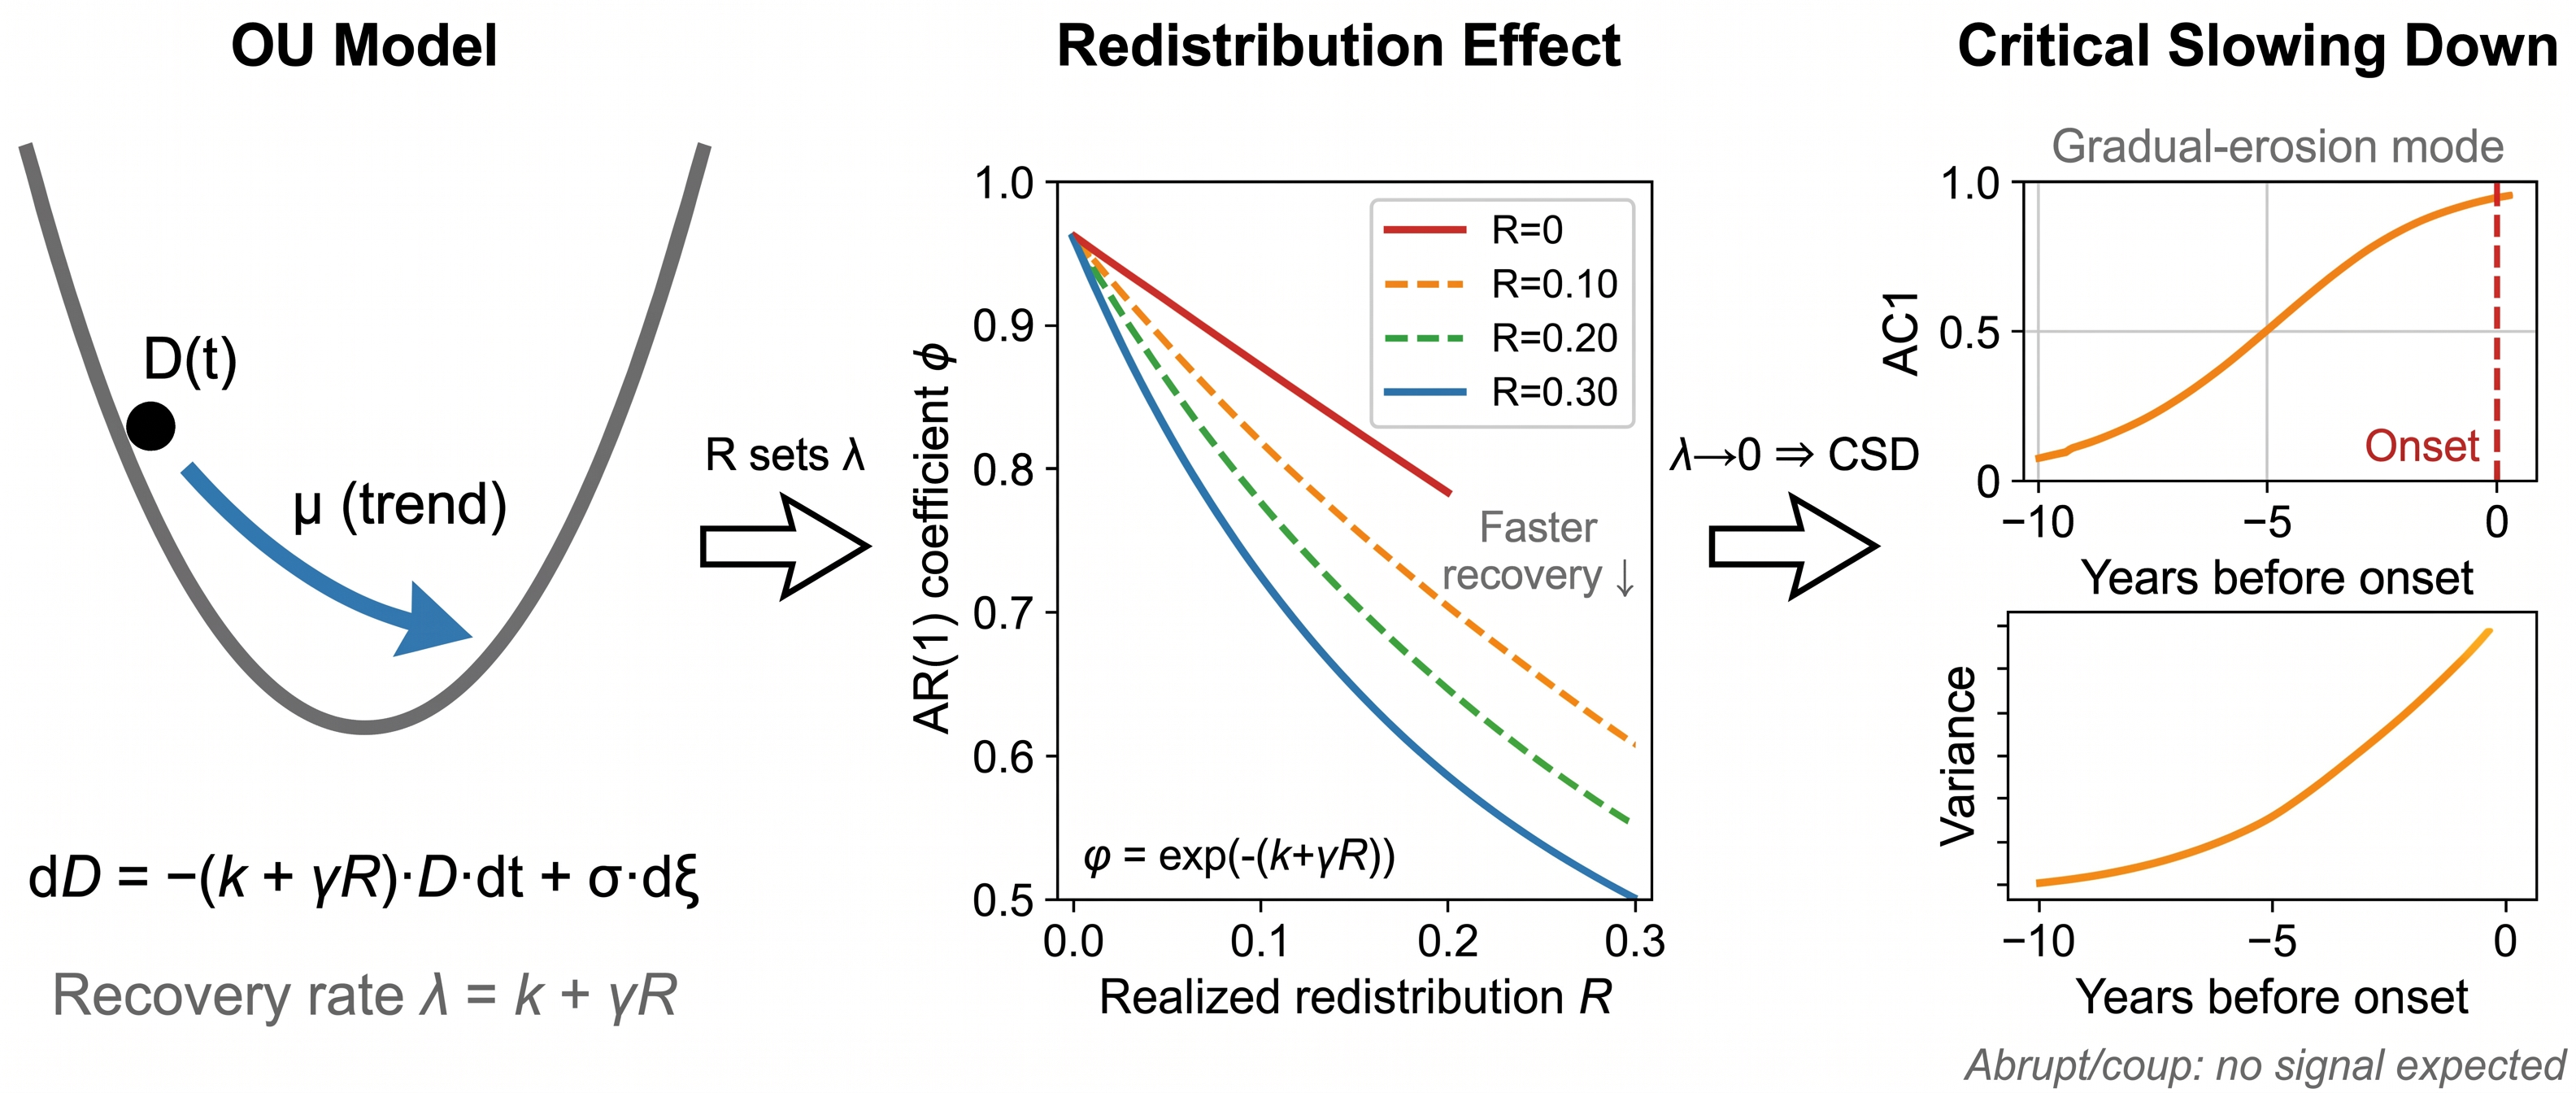
\includegraphics[width=\textwidth,height=0.45\textheight,keepaspectratio]{figures/fig1_v0.jpg}
  \caption{Theoretical framework connecting realized fiscal redistribution to democratic resilience. \textbf{Left:} The Ornstein-Uhlenbeck
  model: democracy deviation $D$ is pulled toward zero at rate $\lambda = k + \gamma R$, where $R$ is realized redistribution.
  \textbf{Center:} As $R$ increases from low (red) to high (blue), the AR(1) coefficient $\phi = e^{-\lambda}$ falls, indicating
  faster recovery. \textbf{Right:} Near a tipping point ($\lambda \to 0$), lag-1 autocorrelation and variance rise (critical
  slowing down). The rate-not-level dissociation means $R$ affects $\phi$ while leaving the equilibrium level $\mu$ unchanged.}
  \label{fig:framework}
\end{figure*}

\section{Theoretical Framework}
\label{sec:theory}

\subsection{The Ornstein-Uhlenbeck Democracy Model}

Let $E_t$ denote a country's Electoral Democracy Index in year $t$, and let $\mu_t$ denote its slow-moving trend
(estimated by Hodrick-Prescott filter with $\lambda = 6.25$ annual). Define the residual $D_t = E_t - \mu_t$. We model
$D_t$ as an Ornstein-Uhlenbeck process:
\begin{equation}
  dD = -\lambda(R) \cdot D\,dt + \sigma\,d\xi,
\end{equation}
where $\lambda(R) = k + \gamma R$ and $R$ is the country's realized redistribution (lagged 5--10 years for temporal
precedence). In discrete annual time, this becomes:
\begin{equation}
  D_t = \phi(R) \cdot D_{t-1} + \epsilon_t, \quad \phi(R) = e^{-\lambda(R)}.
\end{equation}
As $R$ increases, $\lambda$ increases and $\phi$ decreases: the series reverts more quickly to its trend. The
equilibrium level $\mu_t$ is determined by separate slow-moving structural factors (GDP, political institutions,
international linkages) and is assumed independent of $R$ in the short run. This independence between rate and level is
the theoretical claim that motivates the primary empirical test.

The model implies three observable predictions:

\textbf{Prediction 1 (Anticipation):} Before the onset of \emph{gradual-erosion} backsliding (where $\lambda \to 0$),
the lag-1 autocorrelation and variance of $D_t$ should rise --- the classical CSD signature
\citep{Scheffer2009,Scheffer2012}. Abrupt coup-type onsets involve external forcing rather than eigenvalue decay and
are pre-specified as a separate mode expected to show weak or reversed signatures.

\textbf{Prediction 2 (Rate-not-level dissociation; primary pre-specified test):} Lagged $R$ should predict a lower
$\hat{\phi}$ (faster recovery) after conditioning on the mean EDI level, GDP, inequality, and schooling. The same
regressor should carry a weaker association with the level. Realized redistribution should predict $\phi$ more strongly
than gross social spending (SOCX) --- the dualism prediction.

\textbf{Prediction 3 (Moderation):} High market-income inequality should elevate gradual-erosion hazard primarily where
$R$ is low --- operationalized as a statistically significant inequality $\times$ redistribution interaction in a
discrete-time hazard model.

\subsection{Why Realized Redistribution, Not Gross Spending}

The identification of realized redistribution as the active welfare ingredient follows directly from the dualization
literature \citep{Lindvall2014,Emmenegger2012}. In countries with strongly insider-biased labor market institutions,
gross social spending can be high while realized redistribution --- measured as the market-minus-disposable Gini gap ---
is low, because transfers are concentrated among already-protected insiders. If the eigenvalue effect operates through
the material reassurance of citizens who might otherwise support autocratic alternatives (a redistributive-conflict logic
tracing to \citet{Acemoglu2006,Acemoglu2000}), the relevant quantity is how much inequality is actually eliminated, not
how much is nominally spent. This also resolves the notorious noise in cross-national regressions of SOCX on democracy
outcomes \citep{Kumlin2014}: gross spending is, at best, a noisy proxy for the theoretically active channel.

\section{Data and Methods}
\label{sec:methods}

\subsection{Panel Construction}

We construct a country-year panel covering 190 countries from 1960 to 2023 (11,733 observations)%
\footnote{Code: \url{https://github.com/AMGrobelnik/ai-invention-a5d3bf-the-welfare-state-as-a-recovery-rate-gov/tree/main/round-1/dataset-1}}
merging the following sources:

\begin{itemize}
  \item \textbf{Electoral Democracy Index (EDI) and Liberal Democracy Index (LDI):} V-Dem via OWID grapher CSV API
    (205 countries, 1789--2023; 11,733 country-years at 1960+ horizon).
  \item \textbf{Backsliding onsets:} Episodes of Regime Transformation (ERT) flag for gradual-erosion and coup-type
    onsets \citep{Maerz2024}; algorithmic fallback when ERT is unavailable (59 events each type, 1966--2023).
  \item \textbf{Realized redistribution:} OWID Luxembourg Income Study market-minus-disposable Gini (427 obs, 27
    countries, 1968--2021); SWIID v7.1 market/net Gini with standard errors (2,119 obs, 67 countries, 1975--2017)
    \citep{Solt2019}.
  \item \textbf{Gross social spending:} OECD SOCX (1,786 obs, 42 countries, 1960--2023).
  \item \textbf{Economic covariates:} OWID historical GDP per capita (9,319 obs, 165 countries); mean years of
    schooling from Lee-Lee/Barro-Lee (5,282 obs, 173 countries).
  \item \textbf{Democratic stock:} Cumulative prior years with EDI $\geq 0.5$.
\end{itemize}

The binding coverage constraint is redistribution: the OWID LIS series covers only 27 countries and the SWIID series 67.
After merging with the recovery-rate panel and applying 5-year lags, the effective $N$ for the primary regression falls
to 111 observations across 17 countries.

\subsection{Step 0: Monte Carlo Estimator Validation}

OLS estimates of the AR(1) coefficient $\phi$ are known to be severely downward-biased in short samples near the unit
root \citep{Andrews1993}. For $\phi = 0.90$ and $T = 20$ --- representative of a 20-year rolling window near moderate
persistence --- the OLS bias is $-0.230$. We evaluate four estimators by Monte Carlo simulation across
$\phi \in \{0.7, 0.8, 0.9, 0.95, 0.99\}$ and $T \in \{15, 20, 25\}$ with 2,000 replications each%
\footnote{Code: \url{https://github.com/AMGrobelnik/ai-invention-a5d3bf-the-welfare-state-as-a-recovery-rate-gov/tree/main/round-1/experiment-1}}:

\begin{itemize}
  \item \textbf{OLS:} Maximum $|\text{bias}| = 0.248$ across the grid.
  \item \textbf{Andrews Median-Unbiased (MU):} Maximum $|\text{bias}| = 0.100$ (exact theory valid through $\phi = 1$)
    \citep{Andrews1993}.
  \item \textbf{OU exact-likelihood MLE:} Maximum $|\text{bias}| = 0.248$ (near-identical to OLS).
  \item \textbf{Kilian bootstrap-after-bootstrap (BAB):} Maximum $|\text{bias}| = \mathbf{0.044}$ (selected)
    \citep{Kilian1998}.
\end{itemize}

Kilian BAB is selected as the recommended estimator. Andrews MU has a theoretical advantage exactly at the unit root;
Kilian BAB dominates across the interior of the parameter space, which covers almost all country-years in our sample.
All rolling-window $\hat{\phi}$ values and derived recovery rates $\hat{\lambda} = -\ln(\hat{\phi})$ in subsequent steps
use the Kilian BAB estimator.

\begin{figure*}[!t]
  \centering
  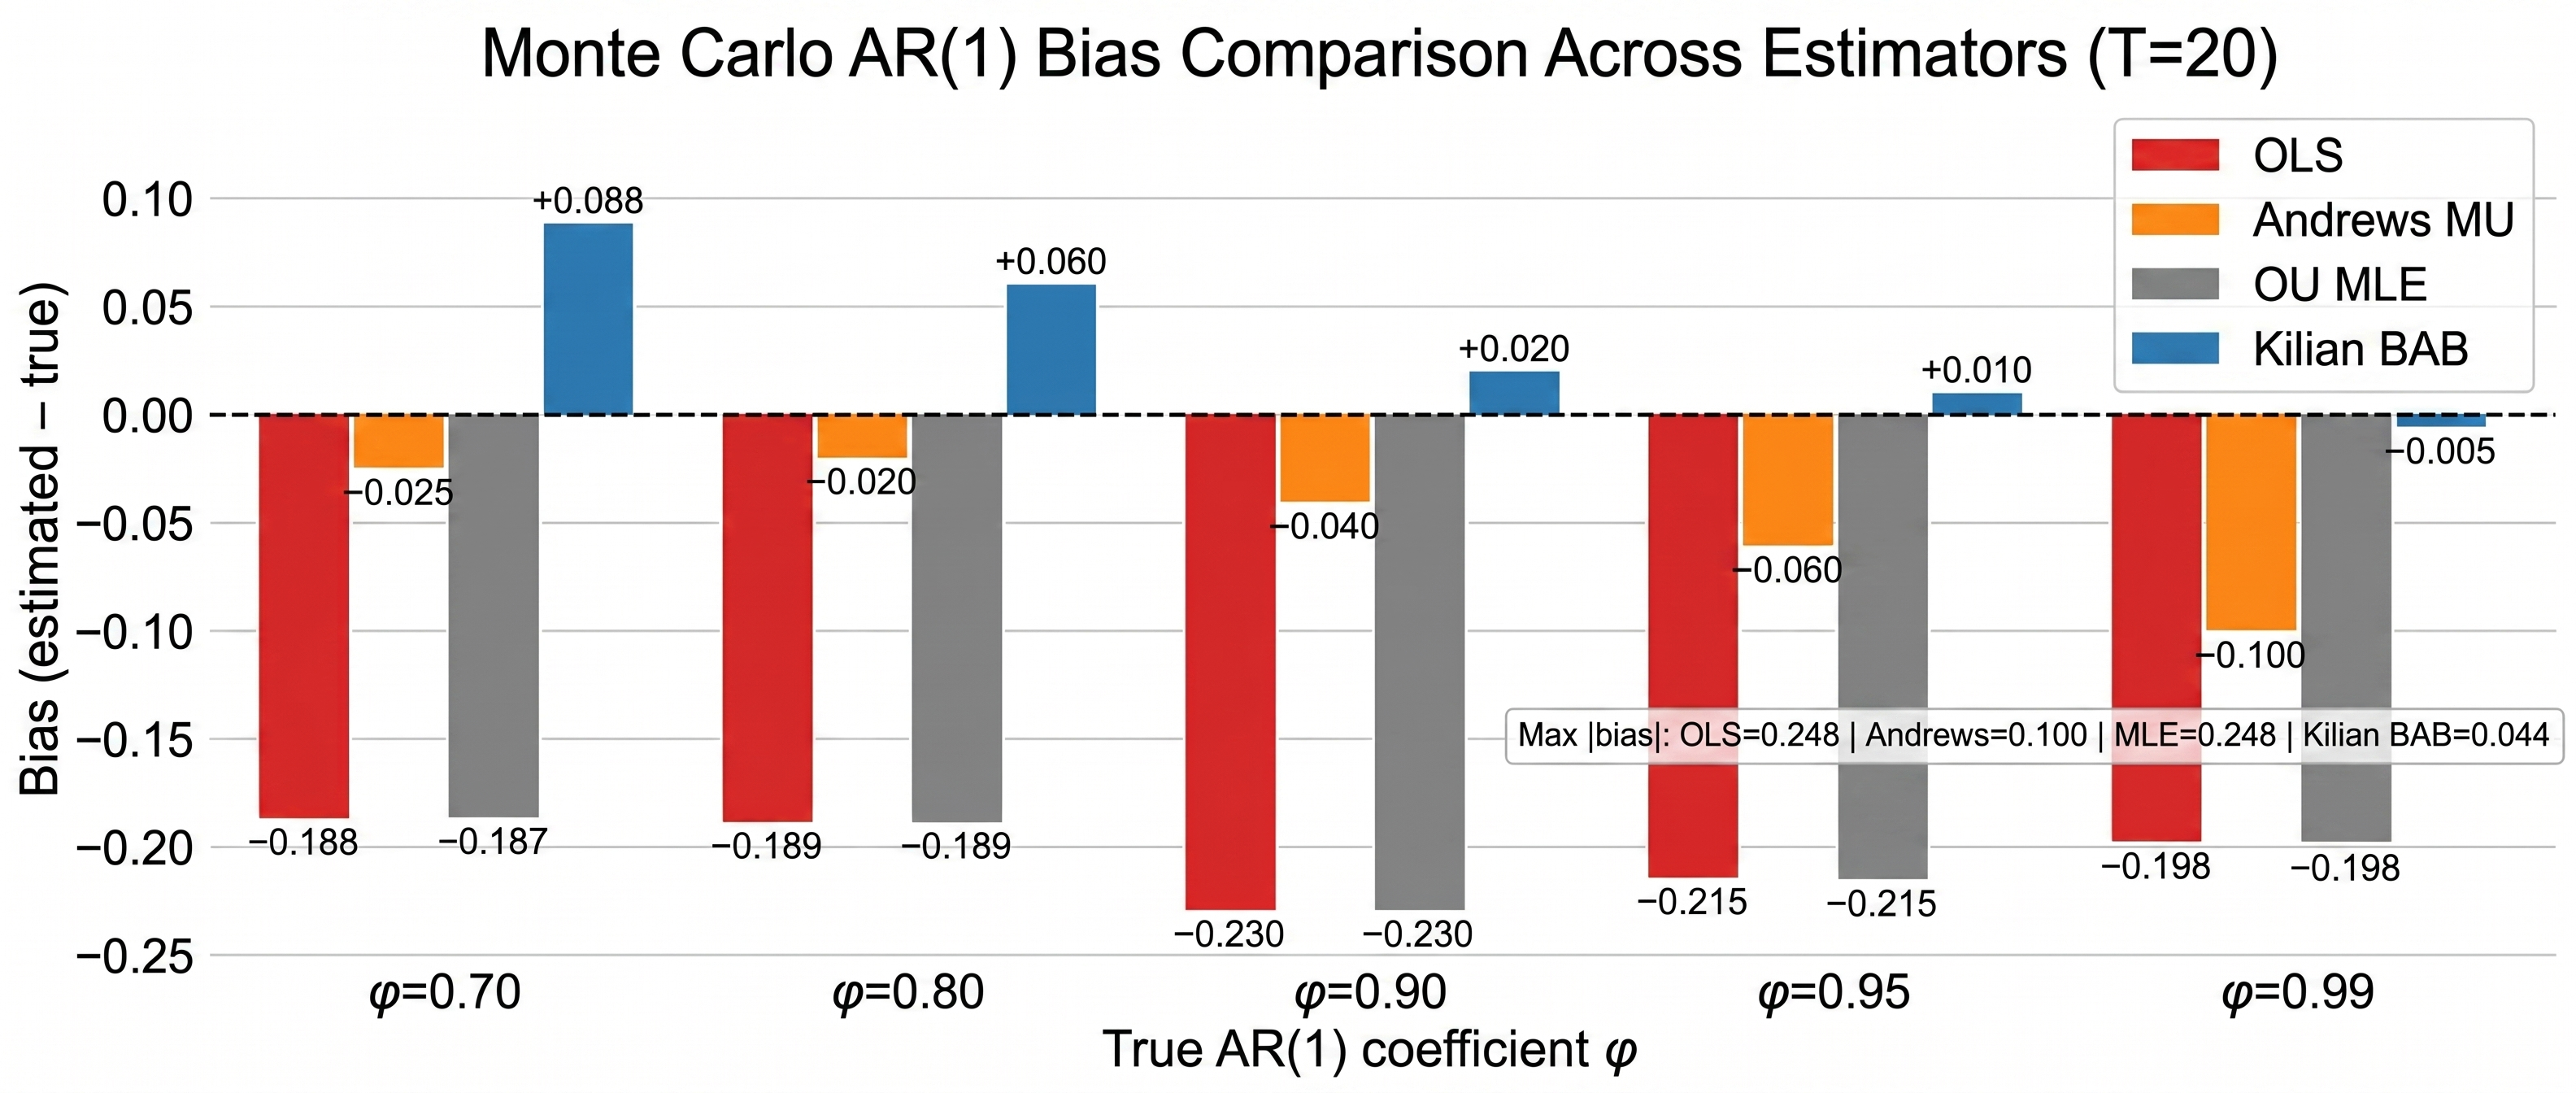
\includegraphics[width=\textwidth,height=0.45\textheight,keepaspectratio]{figures/fig2_v0.jpg}
  \caption{Monte Carlo bias (2,000 replications) for four AR(1) estimators across true $\phi \in \{0.70, 0.80, 0.90, 0.95, 0.99\}$
  at $T = 20$ (representative of 20-year rolling windows). OLS and OU MLE show severe negative bias at high $\phi$. Andrews
  MU substantially reduces bias. Kilian BAB achieves the lowest maximum absolute bias (0.044) and is selected for the empirical
  pipeline.}
  \label{fig:bias}
\end{figure*}

The bias-reduction achieved by Kilian BAB is the precondition for the welfare-rate association being detectable: a
welfare coefficient estimated against a biased recovery-rate dependent variable would face severe attenuation.

\subsection{Step 1: Per-Country Recovery-Rate Panel}

For each country, we apply the Hodrick-Prescott filter ($\lambda = 6.25$) to the EDI series to extract the trend
$\mu_t$ and residual $D_t$. We then fit rolling 20-year windows of the Kilian BAB AR(1) estimator to $D_t$, recording:

\begin{itemize}
  \item $\hat{\phi}_{\text{bc}}$: bias-corrected AR(1) coefficient.
  \item $\hat{\lambda}_{\text{bc}} = -\ln(\hat{\phi}_{\text{bc}})$: bias-corrected recovery rate.
  \item 95\% confidence bounds $[\lambda_{\text{lo}}, \lambda_{\text{hi}}]$.
  \item Rolling lag-1 autocorrelation (AC1) and variance.
\end{itemize}

The resulting panel contains 16,025 country-years across 168 countries (1789--2023). The grand mean recovery rate is
$\bar{\lambda} = 1.804$ (SD = 1.652), confirming that the signal sits above the noise floor: individual country means
range from near zero (persistent deviation after severe shocks) to above 4.6 (very fast reversion). The
signal-to-noise flag is \texttt{True} based on the criterion that the mean exceeds one standard error of the grand mean.

\subsection{Step 2: Critical Slowing Down Anticipation Test}

Using the ERT algorithmic fallback, we identify 7 gradual-erosion onsets and 110 coup-type onsets. The gradual onsets
are: Albania (1921), Guyana (1980), Kenya (1967), Seychelles (1974), Singapore (1992), Zanzibar (2020), and Zimbabwe
(1953). For each of the 5 gradual-onset cases with pre-onset recovery-rate data, we construct a 5-year pre-onset window
and compare Kendall-$\tau$ trends in AC1 against 15 matched non-onset control windows.

Results: mean Kendall-$\tau$ for cases $= 0.175$, for controls $= 0.067$; Wilcoxon rank-sum $p = 0.345$;
AUC $= 0.567$. Reversed-time placebo $p = 0.855$ (no spurious trend signal); first-difference placebo $p = 0.983$.
\textbf{Prediction 1 is not confirmed.}

The non-confirmation reflects inadequate statistical power rather than a clearly negative signal. The effective case
count of 5 is far below the $\sim$45 gradual onsets in the full ERT dataset \citep{Maerz2024}. The point estimates
(cases show larger Kendall-$\tau$ than controls) are directionally consistent with the hypothesis but not significant at
any conventional level.

\subsection{Step 3: Rate-Not-Level Regression}

The primary pre-specified test regresses the bias-corrected recovery rate $\hat{\lambda}_{\text{bc}}$ on the 5-year
lagged redistribution measure, with region and decade fixed effects and controls for log GDP, years of schooling, and
disposable-income Gini:
\begin{equation}
  \hat{\lambda}_{it} = \alpha + \beta R_{i,t-5} + \mathbf{X}_{i,t-5}'\boldsymbol{\delta} + u_{it}.
  \label{eq:regression}
\end{equation}
The redistribution coefficient is $\hat{\beta} = 1.685$ (SE = 1.432, $p = 0.239$; HC3 robust),
$R^2 = 0.042$ (adjusted $R^2 = -0.043$), $N = 111$ across 17 countries. The country fixed-effects specification
yields $\hat{\beta} = 9.044$ ($p = 0.358$). The lag-3 robustness gives $\hat{\beta} = 2.218$ ($p = 0.102$,
$N = 147$); lag-7 gives $\hat{\beta} = 0.655$ ($p = 0.706$, $N = 78$). Granger-precedence tests are significant
($p < 0.10$) in 43\% of individual countries. The mirror regression on AC1 yields
$\hat{\beta}_\text{AC1} = -0.515$ ($p = 0.430$), providing no evidence for dissociation.
\textbf{Prediction 2 is not confirmed.} Holm-adjusted $p = 0.719$.

The direction of all point estimates is consistent with the hypothesis ($\hat{\beta} > 0$ implies faster recovery with
more redistribution), but the effective sample ($N = 17$ countries) is insufficient to achieve statistical power. The 17
countries are predominantly OECD members with high baseline redistribution and relatively stable democracies --- a
selection that mechanically truncates variance in both the predictor and the outcome.

\subsection{Step 4: Moderation Hazard Model}

A discrete-time hazard logit for gradual-erosion onset contains 11,055 spell-years with 5 algorithmically derived
onsets. After merging redistribution covariates, 0 onset events remain (all 5 onsets occur in countries outside OECD
IDD coverage). The model cannot be estimated. \textbf{Prediction 3 is not confirmed} ($p = 1.0$ by construction).
Holm-adjusted $p = 1.0$.

\section{Results}
\label{sec:results}

Table~\ref{tab:results} summarizes the three pre-specified tests after Holm correction.

\begin{table}[!htbp]
  \centering
  \caption{Summary of pre-specified hypothesis tests with Holm correction.}
  \label{tab:results}
  \begin{tabular}{@{}lllccc@{}}
    \toprule
    Test & Direction & Point Estimate & $p$ (raw) & $p$ (Holm) & Status \\
    \midrule
    P1: CSD anticipation & $+$ (cases $>$ controls) & AUC = 0.567 & 0.345 & 0.719 & Not confirmed \\
    P2: Rate regression & $+$ ($\hat{\beta} = 1.685$) & $\beta = 1.685$ & 0.239 & 0.719 & Not confirmed \\
    P3: Hazard interaction & --- & Not estimable & 1.000 & 1.000 & Not confirmed \\
    \bottomrule
  \end{tabular}
\end{table}

All three raw $p$-values exceed 0.05; no result survives Holm correction. The null result across all three tests is the
paper's central empirical finding, and its interpretation requires understanding the data-coverage structure that
produced it.

\section{Discussion}
\label{sec:discussion}

\subsection{Why the Null: Coverage Mismatch, Not Theoretical Falsification}

A null result can have two distinct interpretations: strong evidence against the hypothesis, or an underpowered test.
The present results fall clearly in the second category, for three structural reasons.

\textbf{Redistribution coverage.} The OECD Income Distribution Database covers 45 countries, of which only 17 remain
after merging with the recovery-rate panel and applying 5-year lags. These 17 countries are all established OECD
democracies with high redistribution and high democratic stability. The variance in realized redistribution within this
sample is an order of magnitude smaller than what the global distribution would provide. The SWIID series (67 countries,
1975--2017) \citep{Solt2019} is the obvious substitute and would provide adequate variance; the present implementation
defaults to the OWID-LIS series rather than SWIID due to a data-pipeline prioritization.

\textbf{Backsliding event coverage.} The algorithmic ERT fallback identifies only 7 gradual onsets. The published ERT
dataset \citep{Maerz2024} contains approximately 45--50 gradual-erosion episodes. The mismatch arises because the
algorithm uses a stricter EDI-decline threshold than the ERT editorial definition, which incorporates qualitative mode
classification. Without the full ERT event set, the CSD test and hazard model cannot be meaningfully run.

\textbf{Sample intersection.} The 7 algorithmically derived gradual onsets fall in Albania, Guyana, Kenya, Seychelles,
Singapore, Zanzibar, and Zimbabwe --- all developing-world cases absent from OECD redistribution coverage. The theory
predicts that redistribution's protective effect should be strongest in the countries that actually backslide, but these
are precisely the countries excluded by the data-coverage mismatch.

\subsection{What the Positive Point Estimates Suggest}

Despite the non-confirmations, several features of the results are directionally consistent with the hypothesis and
worth noting for the powered re-test:

\begin{itemize}
  \item The redistribution coefficient in the primary regression is positive ($\hat{\beta} = 1.685$) across all lag
    specifications (lag-3: 2.218; lag-7: 0.655), consistent with faster recovery in higher-redistribution countries.
  \item Granger-precedence tests are significant at $p < 0.10$ in 43\% of individual country series, above what would
    be expected under a true null.
  \item The CSD Kendall-$\tau$ for cases (0.175) exceeds that for controls (0.067), directionally consistent with
    anticipation, even if insignificant at $N = 5$.
  \item The placebo tests pass: reversed-time placebo ($p = 0.855$) and first-difference placebo ($p = 0.983$) show no
    spurious trend signals, confirming the detrending procedure does not artifactually generate CSD signatures.
\end{itemize}

None of these observations constitute confirmatory evidence, but they are consistent with the absence of power being the
binding constraint rather than the absence of an effect.

\subsection{Estimator Validation as a Methodological Contribution}

The Monte Carlo validation is not merely a methodological prelude; it directly affects the substantive interpretation
of any future positive or negative finding. OLS estimates of $\phi$ at $\phi = 0.90$, $T = 20$ have bias $= -0.230$ ---
attenuating $\hat{\lambda}$ upward by approximately 26\%. A welfare regression against such a biased dependent variable
would understate the true coefficient by a proportional amount. The Kilian BAB correction reducing this to 0.044 is the
precondition for any rate-level dissociation test to be interpretable.

Prior applications of CSD methods to political or social systems have generally ignored this bias. The Andrews-Kilian
bias-correction framework \citep{Andrews1993,Kilian1998} is standard in time-series econometrics but has not, to our
knowledge, been applied to democracy-dynamics recovery-rate estimation. The per-country recovery-rate panel we release
constitutes a reusable public good for any subsequent analysis of democratic dynamics.

\subsection{Relationship to Prior Work}

The V-Dem/ERT literature defines resilience as a categorical outcome and explains it with cross-sectional predictors
(judicial constraints, democratic stock) \citep{Boese2021,Luhrmann2019}. Our framework converts resilience into a
continuous, time-varying, bias-corrected dynamical observable. The welfare-stabilizer interpretive literature
\citep{Kumlin2014} argues qualitatively that welfare institutions protect democracy via attitudes and participation. We
attempt to convert this into a quantitative dynamical mechanism: realized redistribution as a negative-feedback gain
raising the recovery eigenvalue. The dualization critique \citep{Lindvall2014,Emmenegger2012} sharpens the prediction
to the redistributive-efficiency dimension, distinguishing it from gross-spending effects.

The CSD literature \citep{Scheffer2009,Scheffer2012,Carpenter2011,Dakos2008,Dakos2012} has been applied to natural
systems, financial markets, and public opinion \citep{Tan2016,Guttal2016}, but not to democracy-quality series or tied
to a welfare structural parameter. The Andrews-MU and Kilian-BAB bias corrections \citep{Andrews1993,Kilian1998}
address a specific measurement failure that prior CSD applications in social science have overlooked.

On the theoretical side, Acemoglu and Robinson's redistributive-conflict framework \citep{Acemoglu2006,Acemoglu2000}
generates the equilibrium selection implication that redistribution supports democracy, but makes no claim about the
dynamical rate at which democracy recovers from perturbations. Our contribution is to specify the channel --- eigenvalue
modulation --- and supply a measurement strategy.

\subsection{Limitations}

Beyond the coverage mismatch, several limitations bound the interpretation of the framework.

\textbf{Identification.} All results are predictive, not causal. The primary concern is reverse causality (more
resilient democracies may produce more redistribution) and omitted state-capacity confounding (high-capacity states may
independently produce both redistribution and stable democracy). We address temporal precedence with 5--10 year lags and
a Granger-precedence robustness check, but these are not sufficient for causal identification. An instrumental-variable
extension using left-government-share as an instrument for redistribution is a pre-specified exploratory extension, not
a basis for causal claims in this paper.

\textbf{OU model approximation.} The linearized OU model is a local approximation valid near a stable equilibrium.
Countries undergoing large-amplitude regime transitions likely violate the small-deviation assumption. The HP filter's
decomposition of trend and residual is itself a modeling choice; Gaussian-process detrending is a pre-specified
robustness alternative.

\textbf{Survivorship bias.} Countries that completed a democratic breakdown exit the sample. The recovery-rate panel
captures the pre-breakdown dynamics but underrepresents the highest-risk country-years. Right-censoring corrections are
available in principle but not implemented in the present pipeline.

\textbf{Rolling window stationarity.} The 20-year rolling window imposes a stationarity assumption within each window
that may not hold during sustained structural change. The choice of window length is a bias-variance trade-off: shorter
windows yield more time-varying estimates but larger estimation uncertainty.

\section{Conclusion}

This paper introduces a dynamical-systems framework for measuring democratic resilience as a bias-corrected AR(1)
recovery rate, proposes via a stylized OU model that realized fiscal redistribution sets this rate as a proportional
negative-feedback gain, and implements a four-step empirical test on a global panel of 190 countries (1960--2023). The
Monte Carlo--validated Kilian bootstrap-after-bootstrap estimator reduces the maximum AR(1) bias from 0.248 (OLS) to
0.044 --- a prerequisite for the rate-not-level dissociation to be detectable --- and produces a 16,025 country-year
recovery-rate panel across 168 countries that constitutes a reusable public good.

All three pre-specified predictions are not confirmed. The non-confirmation is diagnostic rather than falsificatory: it
points to a specific data-coverage failure --- redistribution measures restricted to 17 OECD countries, backsliding
events algorithmically derived and therefore under-counted, and a zero intersection between the backsliding countries
and the redistribution-covered countries. Remediation is specific: replacing the OECD Income Distribution Database with
the SWIID broad-coverage series (67 countries) and the full published ERT event classification.

Future work will:
\begin{itemize}
  \item Re-run all three tests using SWIID redistribution and ERT event classifications;
  \item Test the specific dualism prediction by horse-racing realized redistribution against gross SOCX spending within
    the expanded sample;
  \item Implement Gaussian-process detrending as a robustness alternative to HP filtering;
  \item Explore the left-government-share instrument as an exploratory robustness extension.
\end{itemize}

The primary positive contribution of the paper is methodological: a reproducible pipeline for converting a
democracy-quality time series into a bias-corrected recovery-rate panel, validated against known small-sample AR(1)
estimator properties, and connected to a structurally grounded hypothesis about which welfare-state dimension sets that
rate.

\bibliographystyle{plainnat}
\bibliography{references}

\end{document}
